\documentclass{beamer}

\usepackage{Haust2016glærur}

\title{Tölvunarfræði 1a}
\subtitle{Vika 9, seinni fyrirlestur}

\begin{document}

\begin{frame}
\titlepage
\end{frame}

\section{Inngangur}

\begin{frame}{Í síðasta þætti\ldots}
\begin{itemize}
 \item Innlestur skráa
\end{itemize}
Kafli: 9.3
\end{frame}

\section{Excel-skrár}

\begin{frame}{Excel-skrár}
\begin{itemize}
 \item Matlab getur unnið með Microsoft Excel skrár
 \begin{itemize}
  \item Viðkomandi föll: \texttt{xlswrite} og \texttt{xlsread}
 \end{itemize}
 \item Getur auðveldað flutning gagna á milli kerfa
\end{itemize}
\end{frame}

\begin{frame}[fragile]{\texttt{xlswrite}}
\begin{itemize}
 \item \texttt{xlswrite} skrifar fylki í Excel skrá
 \item Dæmi: Búum til $5 \times 3$ slembifylki og skrifum það í skrána \texttt{ranexcel.xls}
\begin{minted}[frame=lines]{matlab}
>> randomMatrix = randi(100, 5, 3); 
>> xlswrite('ranexcel.xls', randomMatrix); 
\end{minted}
\end{itemize}
\end{frame}

\begin{frame}[fragile]{\texttt{xlsread}}
\texttt{xlsread} les fylki úr Excel-skrá:

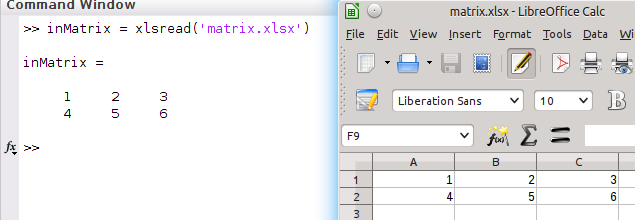
\includegraphics[width=\textwidth]{Pics/excel}

\end{frame}

\begin{frame}{Meira um Excel}
\begin{itemize}
 \item Excel-föllin hafa þó nokkra valkosti sem ekki er farið í hér
 \begin{itemize}
  \item Hægt er að lesa af mismunandi worksheets
  \item \texttt{help xlswrite} og \texttt{help xlsread}!
 \end{itemize}
 \item Til að fá fullan stuðning þarf að vera á Microsoft Windows stýrikerfi, með Microsoft Excel uppsett
 \begin{itemize}
  \item Grundvallarvirkni er þó alltaf til staðar
 \end{itemize}
\end{itemize}
\end{frame}

\section{Að vista breytur í .mat skrár}

\begin{frame}{Save og Load í nýjum buxum}
\begin{itemize}
 \item Hægt er að vista breytur vinnusvæðis í skrá með endinguna \texttt{.mat}
 \begin{itemize}
  \item \texttt{save} skipunin er notuð til að vista breytur í skrána
  \item \texttt{load} skipunin er notuð til að ná í þær aftur
 \end{itemize}
 \item Gagnlegt til að geyma vinnu tímabundið, t.d. til næsta vinnudags
 \item Galli: \texttt{.mat} skrár eru binary-skrár, önnur forrit en Matlab geta ekki lesið þær
\end{itemize}
\end{frame}

\section{Sýnidæmi um skráarvinnslu}

\begin{frame}{Sýnidæmi}
Getum við skrifað forrit sem les gögn og teiknar þau?
\end{frame}

\begin{frame}{Sýnidæmi}
Getum við notað Matlab til að skrifa fyrir okkur heimasíðu?
\end{frame}

\begin{frame}{Fyrirlestraræfing}
Skráið ykkur inn á \url{http://socrative.com/} og klárið æfinguna.

Herbergisnúmer = \texttt{TOL105G2016}

Notendanafn = HÍ-tölvupóstfang
\end{frame}

\end{document}
